\documentclass[12pt,letterpaper]{article}

\usepackage[utf8]{inputenc}

\usepackage{graphicx}
\usepackage{subcaption}

%\usepackage{subfig}         % Multiples imagenes
\usepackage{vmargin}		% Paquete para margenes y formato de página
\setpapersize{A4}
\setmargins	{2.5 cm}     	% margen izquierdo
{0.5 cm}                 	% margen superior
{16.5cm}               		% anchura del texto
{24cm}             		    % altura del texto
{20pt}                		% altura de los encabezados
{1.2cm}               		% espacio entre el texto y los encabezados
{0pt}                		% altura del pie de página
{2cm}                 		% espacio entre el texto y el pie de página

% Preambulo
\usepackage{tikz, tkz-euclide} % hacer gráficos
\usepackage[american, european]{circuitikz} % hacer circuitos
\usepackage{siunitx} % Unidades SI \SI{}{} and \si{} commands for typesetting SI units

\usepackage[spanish, es-tabla, es-noshorthands]{babel}
\usepackage{amsmath}
\usepackage{multirow}
\usepackage{multicol}
\usepackage{tikz, tkz-euclide}
\usetikzlibrary{shapes.geometric, shapes.symbols, arrows, shadows}
\usepackage{graphicx}
\usepackage{float}
\usepackage{booktabs}
\usepackage{circuitikz}
\usepackage{adjustbox}
\usepackage[many]{tcolorbox}
    \tcbuselibrary{theorems}

\usepackage{hyperref}
\usepackage[acronym]{glossaries}
\makeglossaries
%\include{glosario}
\include{acronimos}
\usepackage{biblatex}
\addbibresource{ref.bib}
%\tikzset{>=latex}

\renewcommand{\algorithmicrequire}{\textbf{Input:}}
\renewcommand{\algorithmicensure}{\textbf{Output:}}
\usepackage{listings}
\usepackage{color} %red, green, blue, yellow, cyan, magenta, black, white
\definecolor{mygreen}{RGB}{28,172,0} % color values Red, Green, Blue
\definecolor{mylilas}{RGB}{170,55,241}

\usepackage{pgfplots}
\usetikzlibrary{pgfplots.smithchart}
\usepgfplotslibrary{colorbrewer}
\pgfplotsset{cycle list/Set1-4}
\usepgfplotslibrary{polar}
\pgfplotsset{compat=newest}
\usepgfplotslibrary{smithchart}
\usepackage{siunitx} 
\usepackage{tikz, tkz-base, tkz-fct, pgfplots}
\usepackage{colortbl}
\usepackage{steinmetz}
\usetikzlibrary{bending}
\pgfplotsset{compat=1.13}
\definecolor{micolor}{rgb}{0.9,0.5,0.9}
\ctikzset{current  arrow color/.initial=red}

\usepackage{xparse}
\DeclareDocumentCommand{\newdualentry}{ O{} O{} m m m m } {
  \newglossaryentry{gls-#3}{name={#5},text={#5\glsadd{#3}},
    description={#6},#1
  }
  \makeglossaries
  \newacronym[see={[Glossary:]{gls-#3}},#2]{#3}{#4}{#5\glsadd{gls-#3}}
}


\usepackage{amsmath, amsthm, amsfonts}
\def\RR{\mathbb{R}}
\def\ZZ{\mathbb{Z}}

% De la misma forma se pueden definir comandos con argumentos. Por
% ejemplo, aquí definimos un comando para escribir el valor absoluto
% de algo más fácilmente.
%--------------------------------------------------------------------------

% declaracion de unidades no SI
\DeclareSIUnit{\pf}{pF}
\DeclareSIUnit{\pH}{pH}
\DeclareSIUnit{\nh}{nH}
\DeclareSIUnit{\nf}{nF}
\DeclareSIUnit{\uf}{{\micro}F} 
\DeclareSIUnit{\uh}{{\micro}H} 
\DeclareSIUnit{\ms}{mS}
\DeclareSIUnit{\second}{s}
\DeclareSIUnit{\MHz}{MHz}
\DeclareSIUnit{\dB}{dB}
\graphicspath{ {imagenes/} }

%-----------------------------------------------------------------------------
%               Entorno Para ejemplos 
%-----------------------------------------------------------------------------

 
 %                  Entorno para ecuaciones de ejemplos
 %--------------------------------------------------------------------------
\usepackage{environ}               % Define entornos (ecuaciones de ejemplos)
\NewEnviron{meq}{%
    \begin{equation}
    \scalebox{1}{$\BODY$}           % Se utiliza el paquete "graphix"
    \end{equation}
    }
%------------------------------------------------------------------------------
%                   Entorno de para los diagramas de flujos, como  "Mason"   
%------------------------------------------------------------------------------
\usetikzlibrary{decorations.markings,arrows.meta}
\tikzset
  {midarrow/.style={decoration={markings,mark=at position 0.5 with
     {\arrow[xshift=2pt, purple]{Latex[length=6pt,#1]}}},postaction={decorate}}
  }
  
  \newcommand{\txb}[1]{\small\sffamily #1}
\def\RR{\mathbb{R}}
\def\ZZ{\mathbb{Z}}

%------------------------------------------------------------------------
%           Macros para las redes red1 para grandes (pocos componentes 0-12)
%           pequeños, red2 medianas (varios componentes 0-16)
%           y red3 grandes pequeñas (muchos componentes 0-20)
%-------------------------------------------------------------------------
\newenvironment{red0}[1][0.8]
    {
   \begin{adjustbox}{width=0.4\textwidth}
    \begin{circuitikz}[scale=#1]
    }
    { 
    \end{circuitikz}
   \end{adjustbox} 
    }

\newenvironment{red1}[1][0.7]
    {  \begin{subfigure}[b]{ 0.45\textwidth}
   \begin{adjustbox}{width=0.6\textwidth}
    \begin{circuitikz}[scale=#1]
    }
    { 
    \end{circuitikz}
   \end{adjustbox} 
     \caption{}
    \end{subfigure} 
    }
    
\newenvironment{red2}[1][0.7]{
        \centering
    \begin{subfigure}[b]{0.45\textwidth}
    \begin{adjustbox}{width=0.8\textwidth}
    \begin{circuitikz}[scale=#1]
    }
    { 
    \end{circuitikz}
    \end{adjustbox} 
    \caption{}
    \end{subfigure} 
    }
\newenvironment{red3}[1][0.7]
    {\begin{subfigure}[b]{0.45\textwidth}
    \begin{adjustbox}{width=1\textwidth}
    \begin{circuitikz}[scale=#1]
    }
    { 
    \end{circuitikz}
    \end{adjustbox} 
     \caption{}
    \end{subfigure} 
    }

%------------------------------------------------------------------------
%           Macros para las redes re1 pequeños, rd2 medianos y red3 grandres
%-------------------------------------------------------------------------
\newenvironment{red1a}[1][0.7]{
        
        \begin{adjustbox}{scale=0.8}
        \begin{circuitikz}[scale=#1]
    }
    { 
        \end{circuitikz}
        \end{adjustbox} 
    %\end{center}
    }
    
    \newenvironment{reda}[1][1]
    {\begin{subfigure}[b]{0.4\textwidth}
   \begin{adjustbox}{width=1\textwidth}
    \begin{circuitikz}[x=#1cm,y=#1cm]
    \tikzset{font={\fontsize{15pt}{12pt}\selectfont}}
    %\ctikzset{bipoles/length=25mm}
    \centering
    }
    { 
    \end{circuitikz}
    \end{adjustbox}
    \end{subfigure} 
    }
    
%\ctikzset{bipoles/ammeter/text rotate/.initial=0, rotation/.style={bipoles/ammeter/text rotate=#1},
%}
\newenvironment{redb}[1][0.8]
    {\begin{subfigure}[b]{0.45\textwidth}
   \begin{adjustbox}{width=1\textwidth}
    \begin{circuitikz}[x=0.8cm,y=#1cm]
    \tikzset{font={\fontsize{15pt}{15pt}\selectfont}}
    \ctikzset{bipoles/length=20mm}
    }
    { 
    \end{circuitikz}
    \end{adjustbox} 
     \caption{}
    \end{subfigure} 
    }
%------------------------------------------------------------------------
%          Entorno para los ejemplos
%-------------------------------------------------------------------------
%\usepackage{draftwatermark}
%\SetWatermarkText{\textsc{jpoveda@}} %
% \newtcbtheorem[auto counter, number within = section]{ejemplo}{Ejemplo}%
% 	{   enhanced,
% 	arc=2mm,
% 	interior style={},
% 	attach boxed title to top center= {yshift=-\tcboxedtitleheight/4},
% 	borderline={0.5mm}{0mm}{gray!20!white,dashed},
% 	fonttitle=\bfseries,
% 	fontupper=\itshape,
% 	colbacktitle=white,coltitle=black,
% 	boxed title style={size=normal,colframe=purple!50,boxrule=1pt}
% 	}
% {th}

\newtcbtheorem[auto counter, number within = section]{ejemplo}{Ejemplo CA}%
	{   enhanced,
	arc=2mm,
	interior style={},
	attach boxed title to top center= {yshift=-\tcboxedtitleheight/4},
	borderline={0.5mm}{0mm}{gray!20!white,dashed},
	fonttitle=\bfseries,
	fontupper=\itshape,
	colbacktitle=white,coltitle=black,
	boxed title style={size=normal,colframe=purple!50,boxrule=1pt}
	}
{th}


\usepackage[spanish]{babel} % espanol
\usepackage[latin1]{inputenc} % acentos sin codigo

\title{\textbf{Comunicaciones digitales: Codificación Huffman}}
    \author{Natalia Jimenez Diaz - 20162005243 \\
    Ricardo Andrés Mantilla - 20161005020 \\
    \small Universidad Distrital Francisco José de Caldas\\
    \small Ingeniería electrónica\\
    \small Bogotá
}

\begin{document}

\maketitle

\addtocontents{toc}{\hspace{-7.5mm} \textbf{Capítulos}}
\addtocontents{toc}{\hfill \textbf{Página} \par}
\addtocontents{toc}{\vspace{-2mm} \hspace{-7.5mm} \hrule \par}


\tableofcontents

\maketitle



\maketitle

\newpage

%\input{taller3/taller3}
%\maketitle

\section{Problema}

Realizar un algoritmo en MatLab que demuestre que la informacion mutua de una concatenacion de enlaces de canales binarios es menor que para un solo enlace.

\begin{figure}[H]
    \centering
    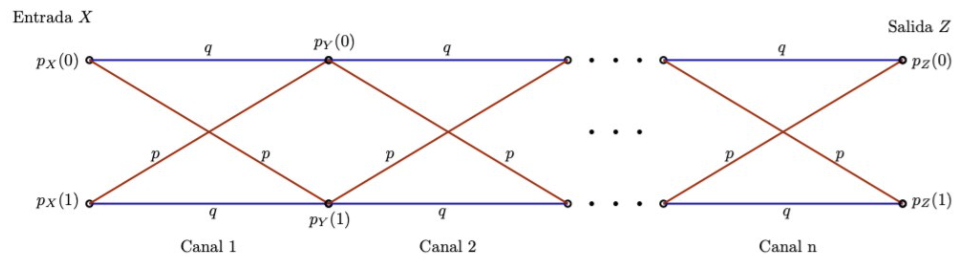
\includegraphics[width=1\textwidth]{taller1/imagenes/canal binario.PNG}
    \caption{\label{fig1}Enlace de comunicaciones}
\end{figure}

\subsection{Solucion}

Para obtener la informacion mutua, se aplica la siguiente ecuacion:

\begin{equation}
    I_{(x;y)}=H_{(x)}-H_{(x|y)}
\end{equation}

Donde:

\begin{equation}
    H_{(x)}=p_{x}\cdot log_{2}(\frac{1}{p_x})
\end{equation}

La incertidumbre promedio viene dada por:

\begin{equation}
    H_{(x|y)}=\sum_{x}\sum_{y}p_{xy(x,y)}\cdot log_{2}(\frac{1}{p_{x|y(x|y)}})
\end{equation}

Para la simulacion de $N$ canales del canal binario, se implementa el siguiente codigo en MatLab.

\begin{figure}[H]
    \centering
    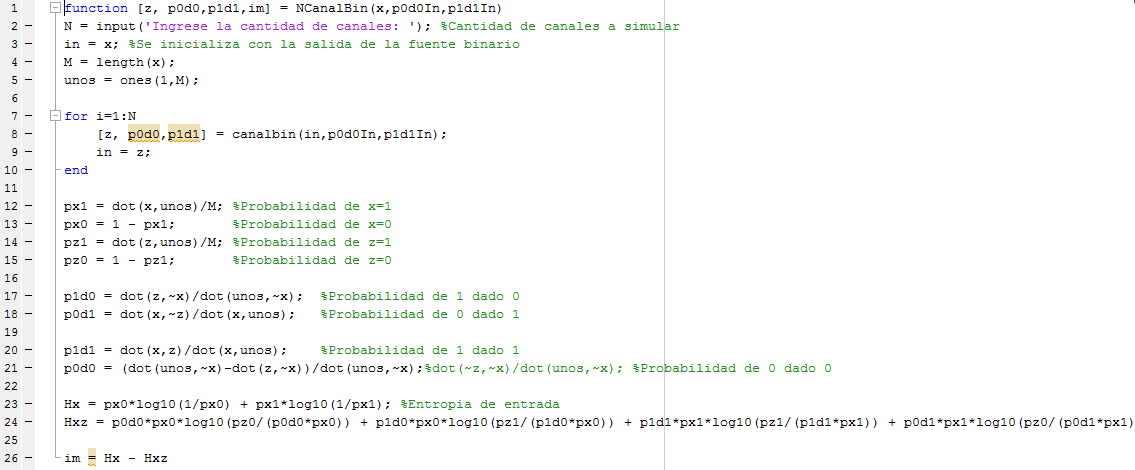
\includegraphics[width=1\textwidth]{taller1/imagenes/codigo canal binario.PNG}
    \caption{\label{fig1}Codigo en Matlab}
\end{figure}

Para este caso, la ecuacion 3 puede ser expresada de la forma:

\begin{equation*}
    H_{(x|y)} = p_{y|x(0|0)}\cdot p_{x(0)}\cdot log_{10}\left(\frac{p_{y(0)}}{p_{y|x(0|0)\cdot p_{x(0)}}}\right)
    +
    p_{y|x(1|0)}\cdot p_{x(0)}\cdot log_{10}\left(\frac{p_{y(1)}}{p_{y|x(1|0)\cdot p_{x(0)}}}\right)+\cdot \cdot \cdot
\end{equation*}

\begin{equation*}
    \cdot \cdot \cdot
    +
    p_{y|x(1|1)}\cdot p_{x(1)}\cdot log_{10}\left(\frac{p_{y(0)}}{p_{y|x(0|1)\cdot p_{x(1)}}}\right)
    +
    p_{y|x(0|1)}\cdot p_{x(1)}\cdot log_{10}\left(\frac{p_{y(0)}}{p_{y|x(0|1)\cdot p_{x(1)}}}\right)
\end{equation*}

Datos que fueron obtenidos en la simulacion, con lo cual se puede determinar la informacion mutua de los $N$ canales.

\subsection{Simulacion}

Se tomaran ciertos casos para comprobar la veracidad del enunciado.
\\
\\
Para $P_{y|x(0|0)} = 0.9$, $P_{y|x(1|1)} = 0.7$ con 1 canal. Simulando varias veces se obtiene un promedio de:

\begin{equation*}
    I_{(x,y)}\approx 0.09352
\end{equation*}

Incrementando los canales a 5:

\begin{equation*}
    I_{(x,y)}\approx 0.00566
\end{equation*}

Ahora con 10 canales:

\begin{equation*}
    I_{(x,y)}\approx 1.1642\cdot 10^{-4}
\end{equation*}

Ahora se obtienen unos valores de las probabilidades de las lineas del canal mas ideales de $P_{y|x(0|0)} = 0.99$, $P_{y|x(1|1)} = 0.99$:

\begin{equation*}
    I_{(x,y)}\approx 0.16826
\end{equation*}

Incrementando los canales a 5:

\begin{equation*}
    I_{(x,y)}\approx 0.0268
\end{equation*}

Ahora con 10 canales:

\begin{equation*}
    I_{(x,y)}\approx 0.00364
\end{equation*}

Se puede destacar una disminucion de $I_{(x,y)}$ a medida que se aumentan los canales, y un aumento a medida que las probabilidades del canal tienden a $1$.

%\maketitle

\section{Laboratorio}

Realizar el diseño y simulacion en SIMULINK del codificador y decodificador MLT-3.

\section{Solución}
\subsection{Diseño del codificador}

\begin{figure}[H]
    \centering
    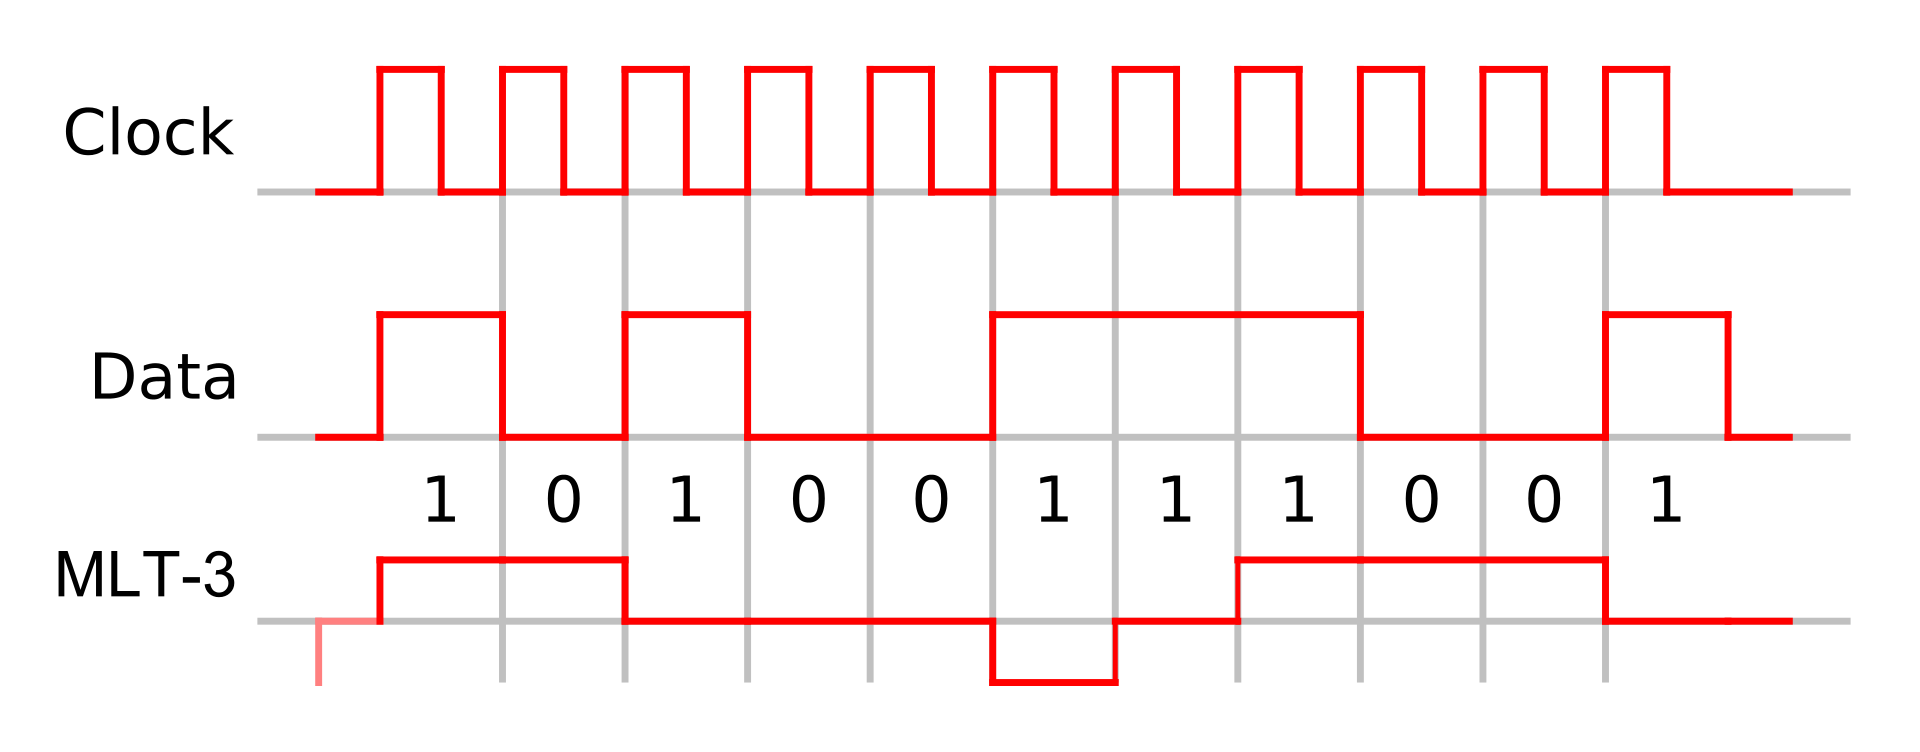
\includegraphics[width=1\textwidth]{laboratorioMLT3/imagenes/MLT3encoding.png}
    \caption{\label{ejemplo}Ejemplo del codificador MLT-3}
\end{figure}

Al analizar el ejemplo de la figura \ref{ejemplo} , se describe que cuando la entrada esta en 0, la salida no presenta cambios, mientras que si esta en 1, la salida cambia entre -1 0 1 dependiendo de su estado anterior, si estaba en -1 o 1, se pasa al estado de 0, mientras que si estaba en 0 se pasa al estado opuesto al ultimo que tuvo, si la señal venia de un -1 ahora pasara a 1 y viseversa. Se explicara mejor el funcionamiento en base al siguiente diagrama de estados de la figura \ref{estados}.

\begin{figure}[H]
    \centering
    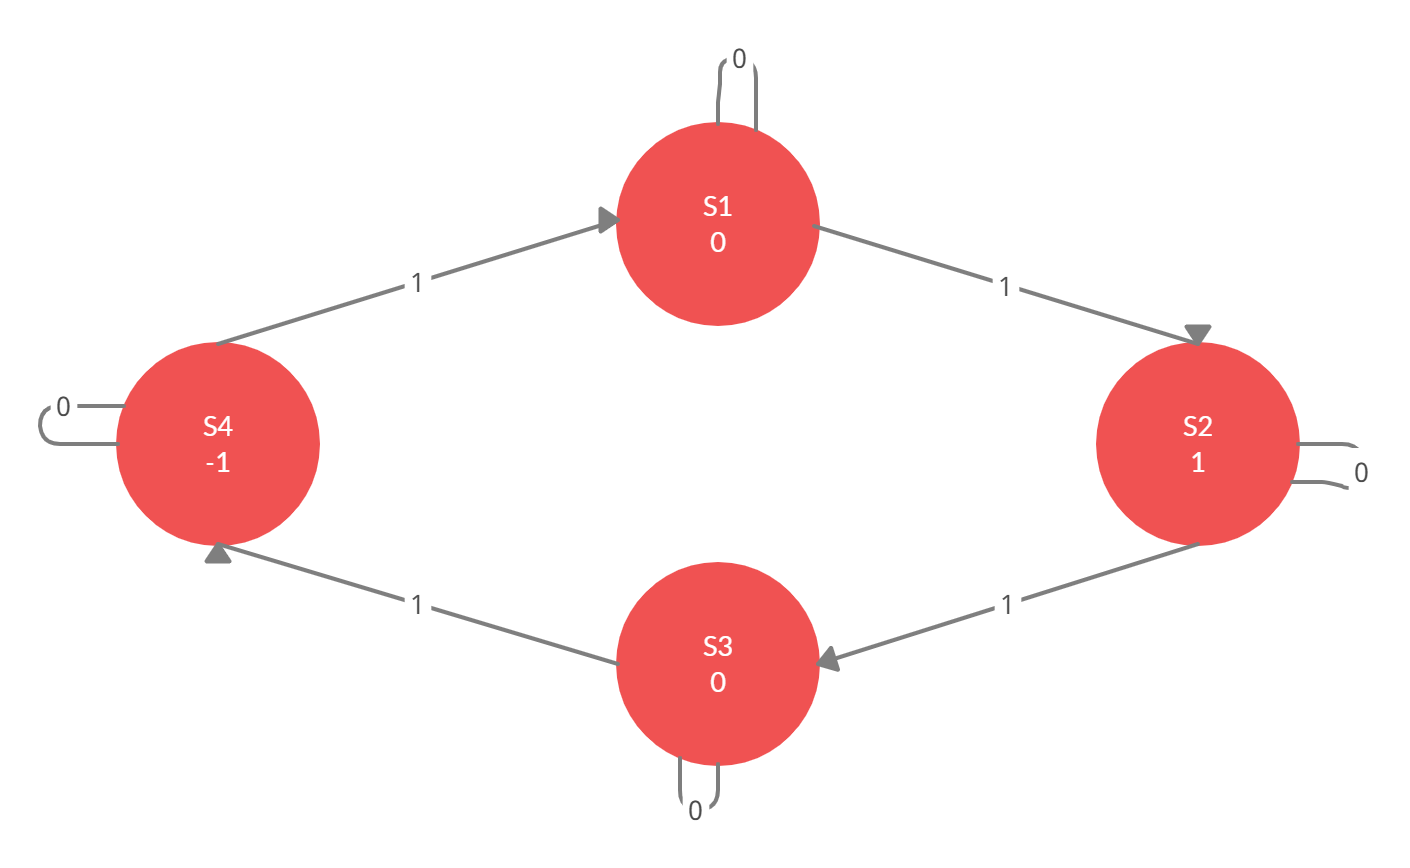
\includegraphics[width=1\textwidth]{laboratorioMLT3/imagenes/Untitled Workspace (1).png}
    \caption{\label{estados}Diagrama de estados}
\end{figure}

Ahora, se especifican las matrices de transicion $T_0$ y $T_1$.
\\
Dado que para entradas en 0 no hay cambios de estado, la matriz de transicion para $T_0$ corresponde a una matriz identidad.

\begin{equation*}
    T_0 = 
    \begin{bmatrix}
        1 & 0 & 0 & 0\\
        0 & 1 & 0 & 0\\
        0 & 0 & 1 & 0\\
        0 & 0 & 0 & 1
    \end{bmatrix}
\end{equation*}

Las entradas en 1 representan cambios al siguiente estado, por lo cual la matriz $T_1$ queda de la forma.

\begin{equation*}
    T_1 = 
    \begin{bmatrix}
        0 & 0 & 0 & 1\\
        1 & 0 & 0 & 0\\
        0 & 1 & 0 & 0\\
        0 & 0 & 1 & 0
    \end{bmatrix}
\end{equation*}

Ya con estas matrices, se procede a implementar la ecuacion de transicion de estados.

\begin{equation*}
    s_{k+1}=[a_{k+1}^*T_0+a_{k+1}T_1]s_k
\end{equation*}

Donde $a_{k+1}$ es la informacion de entrada. $s_k$ viene dada por la siguiente ecuacion.

\begin{equation*}
    s_k = 
    \begin{bmatrix}
        b_k^*e_k^* \\
        b_k^*e_k   \\
        b_ke_k^*   \\
        b_ke_k
    \end{bmatrix}
\end{equation*}

Donde $b_k e_k$ representan los bits de estado del diagrama de estados.\\
Por lo cual la ecuacion de transicion de estados queda de la forma.

\begin{equation*}
    \begin{bmatrix}
        b_{k+1}^*e_{k+1}^* \\
        b_{k+1}^*e_{k+1}   \\
        b_{k+1}e_{k+1}^*   \\
        b_{k+1}e_{k+1}
    \end{bmatrix}
    =
    \left(
    a_{k+1}^*
    \begin{bmatrix}
        1 & 0 & 0 & 0\\
        0 & 1 & 0 & 0\\
        0 & 0 & 1 & 0\\
        0 & 0 & 0 & 1
    \end{bmatrix}
    +
    a_{k+1}
    \begin{bmatrix}
        0 & 0 & 0 & 1\\
        1 & 0 & 0 & 0\\
        0 & 1 & 0 & 0\\
        0 & 0 & 1 & 0
    \end{bmatrix}
    \right)
    \begin{bmatrix}
        b_k^*e_k^* \\
        b_k^*e_k   \\
        b_ke_k^*   \\
        b_ke_k
    \end{bmatrix}
\end{equation*}

Resolviendo las operaciones se obtienen las siguientes cuatro ecuaciones.

\begin{equation}
    \label{eq:1}
    b_{k+1}^*e_{k+1}^*=a_{k+1}^*b_k^*e_k^*+a_{k+1}b_ke_k
\end{equation}

\begin{equation}
    \label{eq:2}
    b_{k+1}^*e_{k+1}=a_{k+1}^*b_k^*e_k+a_{k+1}b_k^*e_k^*=b_k^*(a_{k+1}\oplus e_k)
\end{equation}

\begin{equation}
    \label{eq:3}
    b_{k+1}e_{k+1}^*=a_{k+1}^*b_k e_k^*+a_{k+1}b_k^*e_k
\end{equation}

\begin{equation}
    \label{eq:4}
    b_{k+1}e_{k+1}=a_{k+1}^*b_k e_k+a_{k+1}b_k e_k^*=b_k(a_{k+1}\oplus e_k)
\end{equation}

Ahora se busca obtener el valor de $b_{k+1}$ y $e_{k+1}$, para ello se suman las ecuaciones \ref{eq:3} y \ref{eq:4} lo cual permite obtener la ecuacion de $b_{k+1}$, quedando de la forma.

\begin{equation*}
    b_{k+1}=a_{k+1}^*b_k+a_{k+1}(b_k\oplus e_k)
\end{equation*}

Para obtener la ecuacion de $e_{k+1}$, se suman las ecuaciones \ref{eq:2} y \ref{eq:4}.

\begin{equation*}
    e_{k+1}=a_{k+1}\oplus e_k
\end{equation*}

\subsection{Simulacion del codificador}

Se implementan las ecuaciones del diseño del encoder tal como se muestra en la figura \ref{coder}.

\begin{figure}[H]
    \centering
    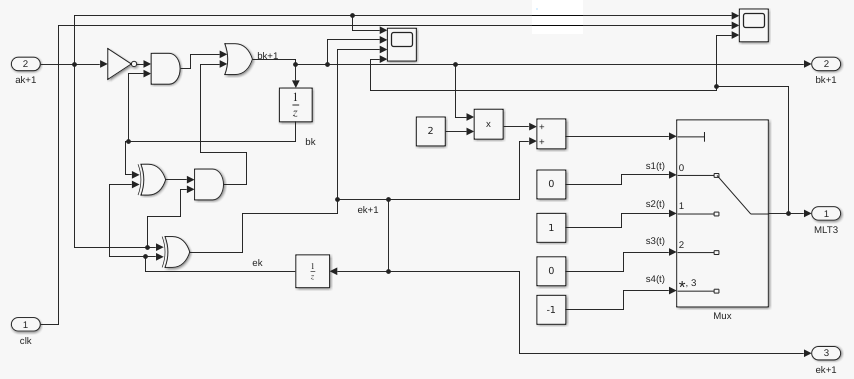
\includegraphics[width=1\textwidth]{laboratorioMLT3/imagenes/coder.PNG}
    \caption{\label{coder}Circuito del codificador}
\end{figure}

Lo cual da la siguiente salida del codificador tal como se ve en la figura \ref{sico}.

\begin{figure}[H]
    \centering
    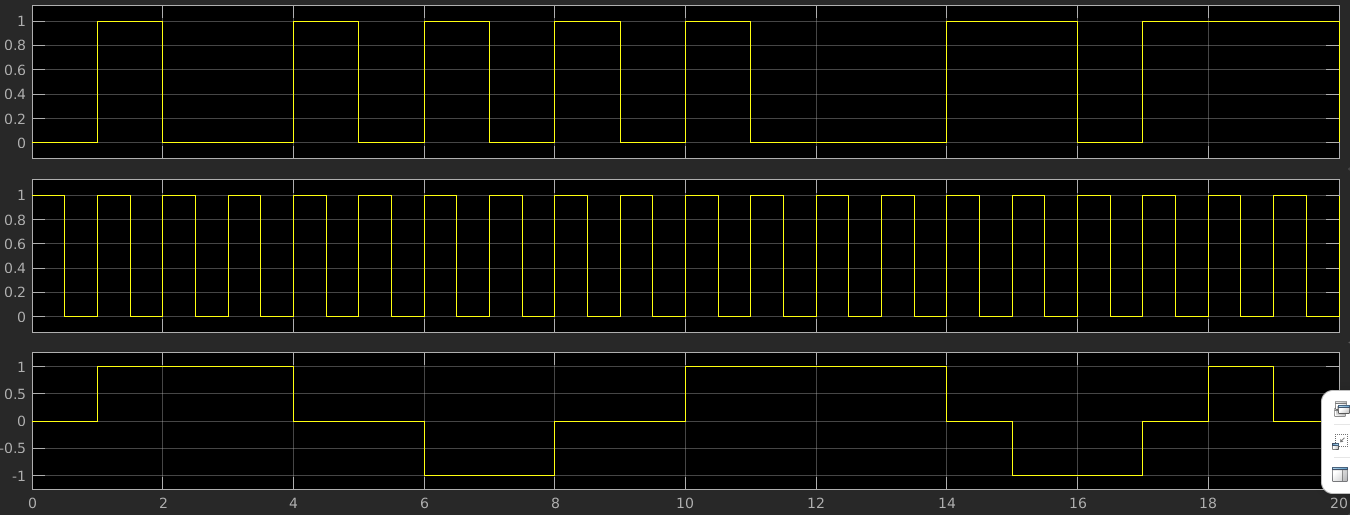
\includegraphics[width=1\textwidth]{laboratorioMLT3/imagenes/simulacionCoder.PNG}
    \caption{\label{sico}Simulacion del codificador}
\end{figure}

La primera grafica corresponde a la señal transmitida, la segunda grafica corresponde al reloj, la tercera es la salida del codificador.

\begin{figure}[H]
    \centering
    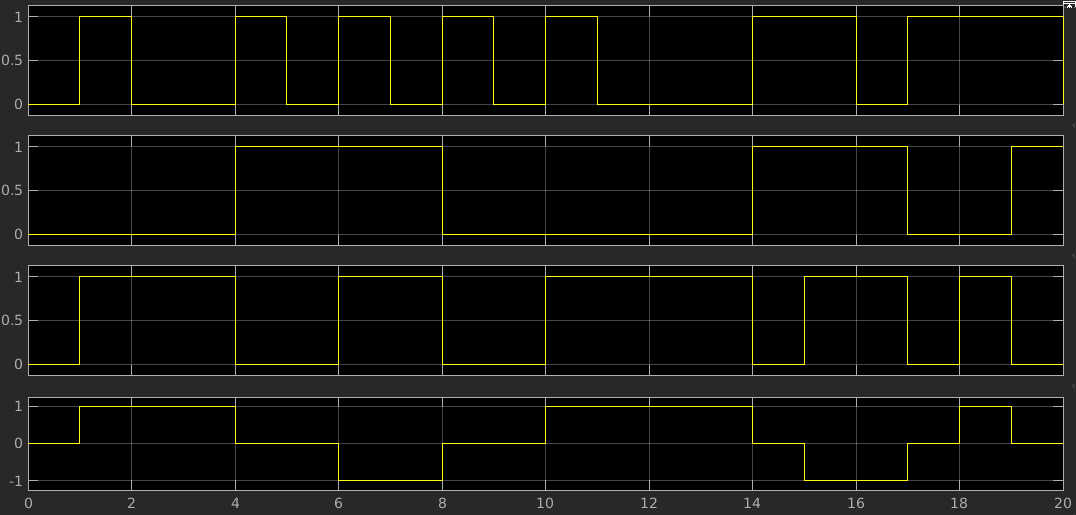
\includegraphics[width=1\textwidth]{laboratorioMLT3/imagenes/simulacionCoder2.PNG}
    \caption{\label{sico2}Simulacion del codificador}
\end{figure}

La figura \ref{sico2} tiene la señal de entrada, la señal $b_{k+1}$ y $e_{k+1}$ que representan las señales de estado, y la señal de salida del codificador.

\subsection{Diseño del decodificador}

Para el diseño del decodificador, se basara en capturar la señal emitida por el codificador y en base a sus estados, se obtendra la señal original de entrada.\\
La figura \ref{deco} explica el funcionamiento de la maquina de estados que permitira decodificar la señal.

\begin{figure}[H]
    \centering
    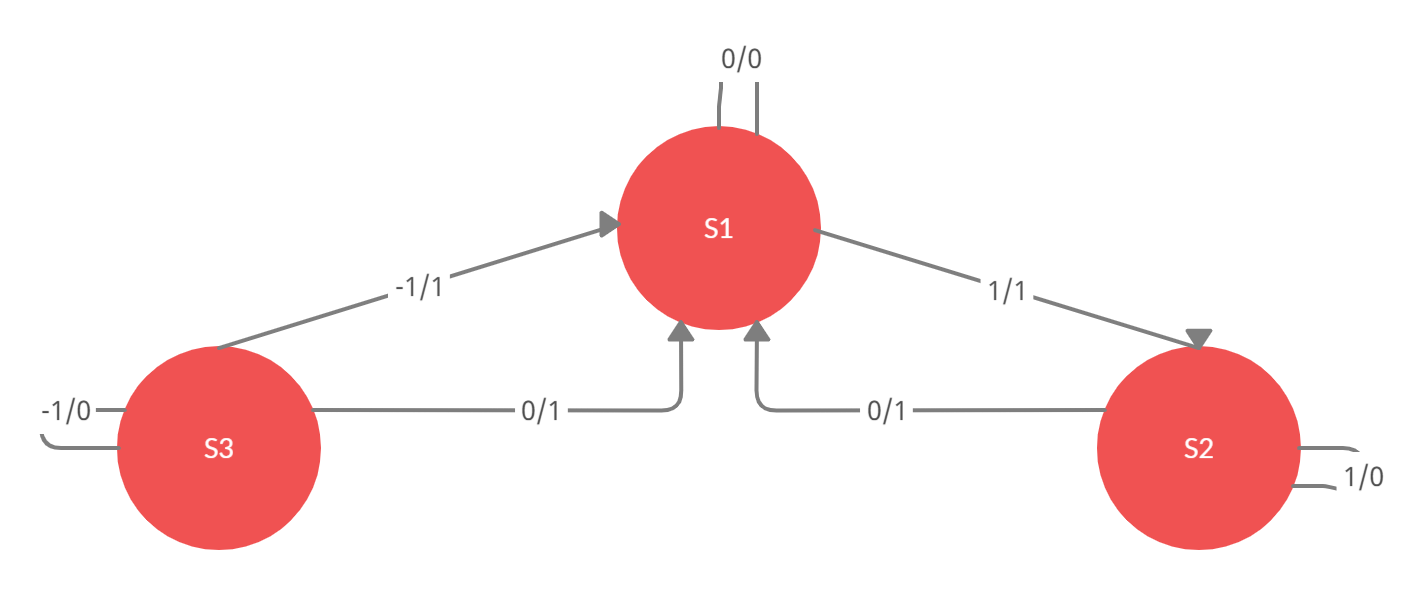
\includegraphics[width=1\textwidth]{laboratorioMLT3/imagenes/Untitled Workspace (2).png}
    \caption{\label{deco}Diagrama de estados del decodificador}
\end{figure}

Donde la salida depende del cambio de estados y permite obtener la señal decodificada.\\
El codificador emite señales con los valores de $0$ $1$ y $-1$, por lo cual el $-1$ se representara como un 2 binario. Ya teniendo una señal binaria, el bit mas significativa va representado por $x_0$ y el menos significativo por $x_1$. La tabla de estados se especifica a continuacion.

\vspace{0.6cm}
\begin{tabular}{| c | c | c | c | c | c | c |}
\hline
 $s_a$ & $s_b$ & $x_0$ & $x_1$ & $s_{a+1}$ & $s_{b+1}$ & $a_{k+1}$\\ \hline
0 & 0 & 0 & 0 & 0 & 0 & 0 \\
0 & 0 & 0 & 1 & 0 & 1 & 1 \\
0 & 0 & 1 & 0 & 1 & 0 & 1 \\
0 & 0 & 1 & 1 & x & x & x \\
0 & 1 & 0 & 0 & 0 & 0 & 1 \\
0 & 1 & 0 & 1 & 0 & 1 & 0 \\
0 & 1 & 1 & 0 & x & x & x \\
0 & 1 & 1 & 1 & x & x & x \\
1 & 0 & 0 & 0 & 0 & 0 & 1 \\
1 & 0 & 0 & 1 & x & x & x \\
1 & 0 & 1 & 0 & 1 & 0 & 0 \\
1 & 0 & 1 & 1 & x & x & x \\
\hline
\end{tabular}
\vspace{0.2cm}

Basados en la tabla anterior, se obtuvieron las siguientes ecuaciones.

\begin{equation*}
    s_{a+1}=x_0
\end{equation*}

\begin{equation*}
    s_{b+1}=x_1
\end{equation*}

\begin{equation}
    \label{eq:deco}
    a_{k+1} = (s_b\oplus x_1)+(s_a\oplus x_0)
\end{equation}

\subsection{Simulacion del decodificador}

Se implementan las ecuaciones obtenidas en el diseño, tal como se muestra en la figura \ref{decoSimu}.

\begin{figure}[H]
    \centering
    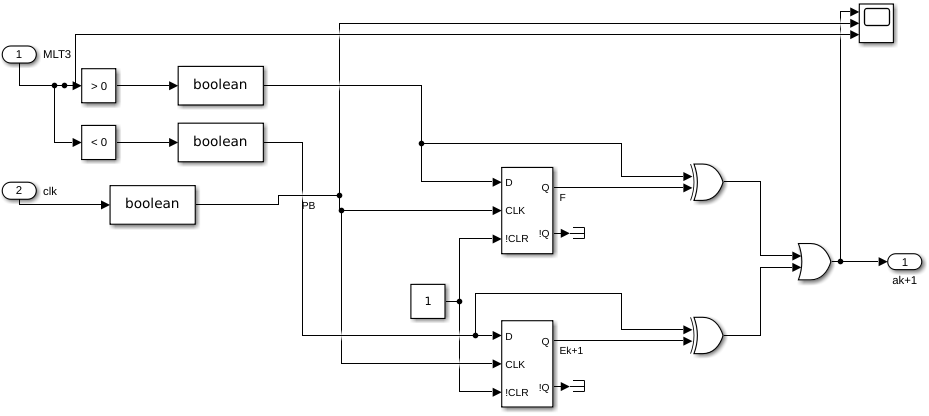
\includegraphics[width=1\textwidth]{laboratorioMLT3/imagenes/decoder.PNG}
    \caption{\label{decoSimu}Circuito del decodificador}
\end{figure}

Primero se transforma la señal del codificador a binario mediante el uso de comparadores que permiten separar cada bit, los cuales se le asignan a cada flip flop tipo D, luego se aplica la ecuacion \ref{eq:deco} para poder obtener la señal decodificada.\\
\\
Se obtiene la siguiente simulacion.

\begin{figure}[H]
    \centering
    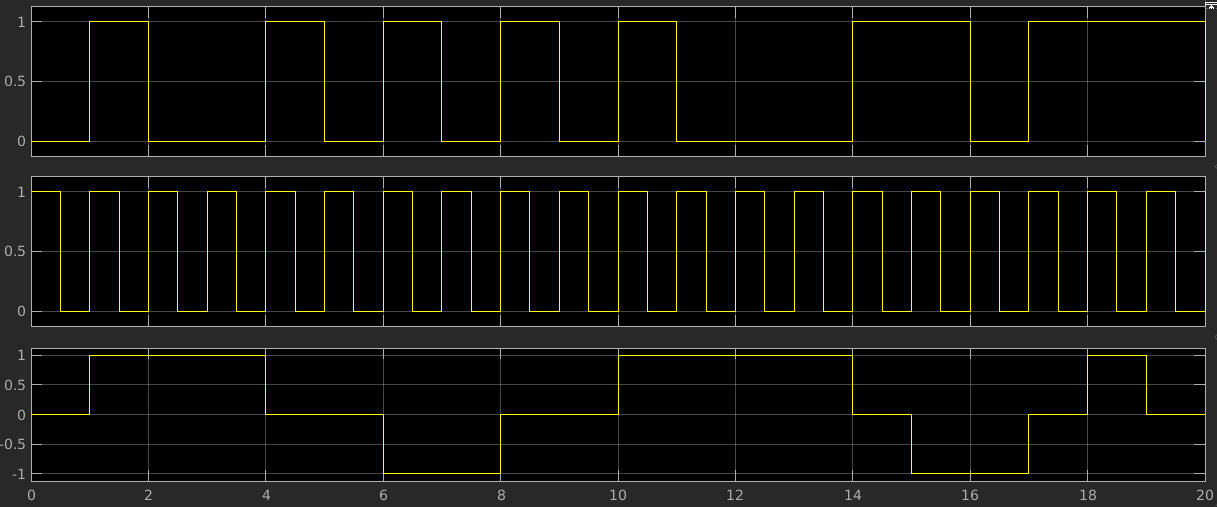
\includegraphics[width=1\textwidth]{laboratorioMLT3/imagenes/simulacionDecoder.PNG}
    \caption{\label{}Simulacion del decoder}
\end{figure}

Donde la primera grafica es la salida del decodificador, la segunda el reloj y la tercera es la entrada del decodificador.

\subsection{Resultados}

Finalmente el circuito queda de la siguiente forma

\begin{figure}[H]
    \centering
    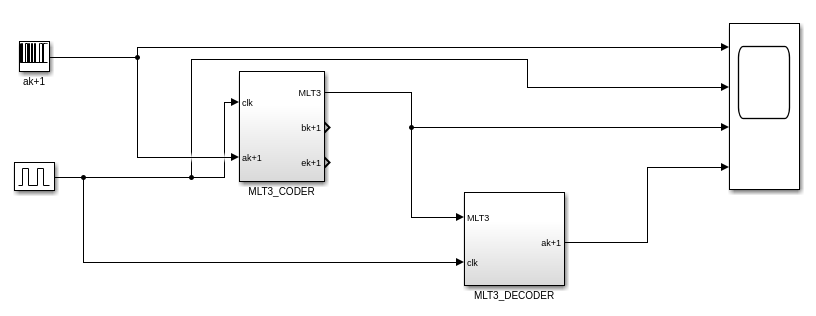
\includegraphics[width=1\textwidth]{laboratorioMLT3/imagenes/circuitoFinal.PNG}
    \caption{\label{}Circuito final}
\end{figure}

Se simula el circuito.

\begin{figure}[H]
    \centering
    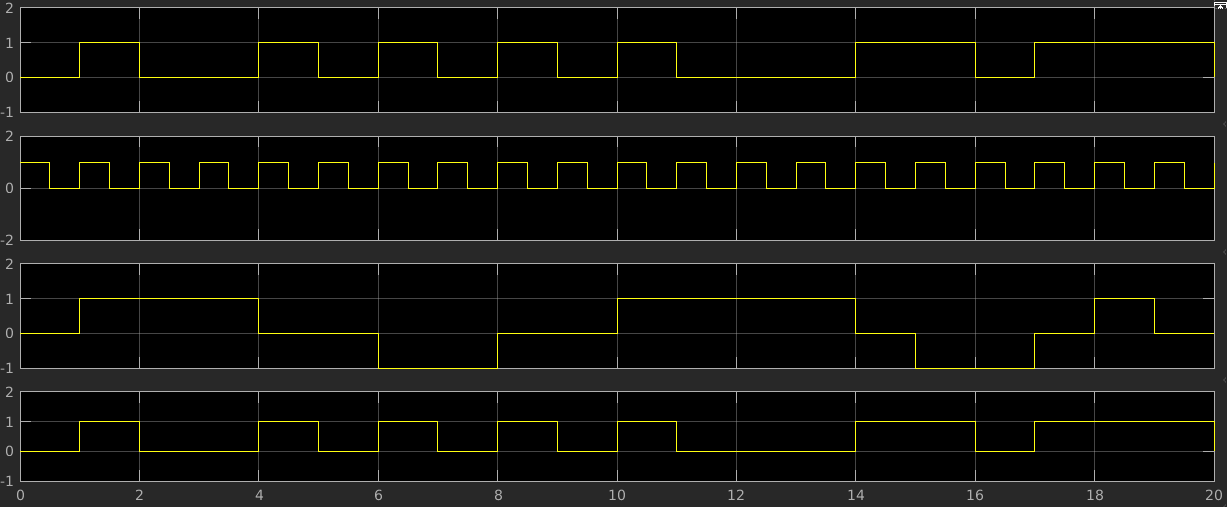
\includegraphics[width=1\textwidth]{laboratorioMLT3/imagenes/simulacionFinal.PNG}
    \caption{\label{}Simulacion final}
\end{figure}

La primera grafica corresponde a la señal a enviar, la segunda el reloj, la tercera es la salida del codificador y la cuarta es la salida del decodificador.
\maketitle

\section{Laboratorio}
Realizar el algoritmo del codificador y decodificador para la codificación Huffman mediante el software de Matlab.

\section{Solución}
\subsection{Codificador}

\lstset{language=Matlab,%
    %basicstyle=\color{red},
    breaklines=true,%
    morekeywords={matlab2tikz},
    keywordstyle=\color{blue},%
    morekeywords=[2]{1}, keywordstyle=[2]{\color{black}},
    identifierstyle=\color{black},%
    stringstyle=\color{mylilas},
    commentstyle=\color{mygreen},%
    showstringspaces=false,%without this there will be a symbol in the places where there is a space
    numbers=left,%
    numberstyle={\tiny \color{black}},% size of the numbers
    numbersep=9pt, % this defines how far the numbers are from the text
    emph=[1]{for,end,break},emphstyle=[1]\color{red}, %some words to emphasise
    %emph=[2]{word1,word2}, emphstyle=[2]{style},    
}

Inicialmente, se implementa el siguiente codigo.

\begin{lstlisting}[language=Matlab,breaklines = true,frame      = false]
   mensaje = fopen(in); % file open
   lectura = fscanf(mensaje,'%c'); % Se lee la data del archivo
   tamanioLectura = length(lectura); % Cantidad de caracteres del archivo
   toAscii = double(lectura); % Se convierten las letras a numeros por ascii
   inAscii = 32; % espacio
   endAscii = 126; % ~
   
\end{lstlisting}

Donde $in$, es un archivo de tipo .txt que contiene un mensaje en texto. Se lee el contenido del archivo y se convierten las palabras a el código Ascii. Se analizaran los caracteres del código Ascii imprimibles, los cuales van desde 'espacio' = 32 hasta 126 = \~  .

\begin{lstlisting}[language=Matlab,breaklines = true,frame      = false]
   proLetras = []; % Probabilidad de cada letra
   
   % Calculo de las probabilidades
   for i=inAscii:endAscii % Desde el espacio hasta la z
       proLetras = [proLetras,length(find(toAscii==i))/tamanioLectura]; % Se aniade su probabilidad
   end
   
\end{lstlisting}

Luego se calcula la probabilidad de que salga un carácter en el texto, para lo cual se cuentan la cantidad de veces que aparece cada carácter y se divide por la cantidad de carácteres.

\begin{lstlisting}[language=Matlab,breaklines = true,frame      = false]
   [dic,M] = Huffman_Dict(proLetras);% Diccionario
   ldic = length(dic);
   dic2 = [];
   a = '';

   % Se convierten los datos del diccionario a texto
    for i=1:ldic    
        for j=1:length(dic(i).a)        
            a = strcat(a,string(dic(i).a(j)));
        end
        dic2=[dic2,string(a)];
        a='';
    end
   
\end{lstlisting}

Ahora, en base a las probabilidades calculadas, se usa la función de $Huffman\_Dict()$ entregada por el profesor, para obtener el diccionario, luego se convierten los datos del diccionario a tipo String para facilitar su manejo.

\begin{lstlisting}[language=Matlab,breaklines = true,frame      = false]
    textoCodificado = '';

    % Se busca cada letra del mensaje y se guarda con su valor del
    %diccionario
    for i=1:length(toAscii)
        textoCodificado = strcat(textoCodificado,string(dic2(toAscii(i)-(inAscii-1))));
    end

    % Se convierte de String a vector de char
    codificado = convertStringsToChars(textoCodificado);
    diccionario = dic2;
   
\end{lstlisting}

Finalmente, se recorre el mensaje a transmitir, donde se buscara cada carácter y se busca su representación en el diccionario, para finalmente concatenarlo a la salida del codificador.\\
La salida del codificador sera la señal codificada y el diccionario.

\subsection{Decodificador}

El código del decodificador se muestra a continuación.

\begin{lstlisting}[language=Matlab,breaklines = true,frame      = false]
    function[out] = Huffman_Deco(in,dic)

    % in: entrada de datos binaria
    % dic: diccionario
    
    lin = length(in);
    a = '';
    mensaje = [];
    
    for i=1:lin
        a = strcat(a,in(i)); % Se concatena la codificacion de a un bit
        if find(dic==a) % Se analiza si lo concatenado existe en el diccionario
            mensaje = [mensaje,find(dic==a)+31];
            a='';
        end
    end
    
    out = char(mensaje);
   
\end{lstlisting}

Para el decodificador, simplemente se recorre la señal codificada bit a bit y se va concatenando cada bit a una variable, por cada bit añadido, se busca si lo que se lleva concatenado existe en el diccionario, si existe, se analiza a que carácter pertenece y se concatena en la señal de salida, y se sigue el mismo procedimiento hasta finalizar el texto codificado.


    
\end{document}